\documentclass[10pt,twocolumn,letterpaper]{article}

\usepackage{cvpr}
\usepackage{times}
\usepackage{epsfig}
\usepackage{graphicx}
\usepackage{amsmath}
\usepackage{amssymb}
\usepackage{pdfpages}

%%%%%%%%%
% Example of figure inclusion
%\begin{figure}[t]
%\begin{center}
%\fbox{\rule{0pt}{2in} \rule{0.9\linewidth}{0pt}}
%   %\includegraphics[width=0.8\linewidth]{egfigure.eps}
%\end{center}
%   \caption{Example of caption.  It is set in Roman so that mathematics
%   (always set in Roman: $B \sin A = A \sin B$) may be included without an
%   ugly clash.}
%\label{fig:long}
%\label{fig:onecol}
%\end{figure}

%%%%%%%%%
% Example table
%\noindent
%Compare the following:\\
%\begin{tabular}{ll}
% \verb'$conf_a$' &  $conf_a$ \\
% \verb'$\mathit{conf}_a$' & $\mathit{conf}_a$
%\end{tabular}\\
%
%
%
%\begin{table}
%\begin{center}
%\begin{tabular}{|l|c|}
%\hline
%Method & Frobnability \\
%\hline\hline
%Theirs & Frumpy \\
%Yours & Frobbly \\
%Ours & Makes one's heart Frob\\
%\hline
%\end{tabular}
%\end{center}
%\caption{Results.   Ours is better.}
%\end{table}

%%%%%%%%%
% another example figure
%\begin{figure*}
%\begin{center}
%\fbox{\rule{0pt}{2in} \rule{.9\linewidth}{0pt}}
%\end{center}
%   \caption{Example of a short caption, which should be centered.}
%\label{fig:short}
%\end{figure*}
%
%
%%%%%%%%%
% example citation
%   Frobnication has been trendy lately.
%   It was introduced by Alpher~\cite{Alpher02}, and subsequently developed by
%   Alpher and Fotheringham-Smythe~\cite{Alpher03}, and Alpher \etal~\cite{Alpher04}.''

    %Figure and table captions should be 9-point Roman type as in
    %Figures~\ref{fig:onecol} and~\ref{fig:short}.  Short captions should be centred.
% Include other packages here, before hyperref.

% If you comment hyperref and then uncomment it, you should delete
% egpaper.aux before re-running latex.  (Or just hit 'q' on the first latex
% run, let it finish, and you should be clear).
%
% When placing figures in \LaTeX, it's almost always best to use
% \verb+\includegraphics+, and to specify the  figure width as a multiple of
% the line width as in the example below
% {\small\begin{verbatim}
%    \usepackage[dvips]{graphicx} ...
%       \includegraphics[width=0.8\linewidth]
%           {myfile.eps}
%   \end{verbatim}
% }
%
\usepackage[breaklinks=true,bookmarks=false]{hyperref}

\cvprfinalcopy % *** Uncomment this line for the final submission

\def\cvprPaperID{****} % *** Enter the CVPR Paper ID here
\def\httilde{\mbox{\tt\raisebox{-.5ex}{\symbol{126}}}}

% Pages are numbered in submission mode, and unnumbered in camera-ready
%\ifcvprfinal\pagestyle{empty}\fi
\setcounter{page}{1}
\begin{document}

%%%%%%%%% TITLE
\title{Predicting the Eye Fixations with Prior Knowledge: A Bayesian Learning Architecture}

\author{Lauren Arnett and Chengzhi Mao\\
Columbia University in the City of New York\\
    {\tt\small \{lba2138,cm3797\}@columia.edu}
}

\maketitle

%%%%%%%%% ABSTRACT
\begin{abstract}
   Applications of tracking eye fixation location span from neuroscience and
   the study of human vision to advertising and human computer interaction. 
   We look to improve upon existing models of saliency. 

\end{abstract}

%%%%%%%%% BODY TEXT
\section{Introduction}

Please follow the steps outlined below when submitting your manuscript to
the IEEE Computer Society Press.  This style guide now has several
important modifications (for example, you are no longer warned against the
use of sticky tape to attach your artwork to the paper), so all authors
should read this new version.

%-------------------------------------------------------------------------
\section{Related Work}

\section{Dataset of Eye-Tracking Data}
\section{Learning a Model}
\subsection{Baseline Model Setting}
We conduct a binary classification task for each output pixel in our baseline eye fixation model. We propose a U-Net architecture, using a fixed pretrained VGG model. We take the features of 3, 8, 15, 22 layers in the VGG and feed into our fixation prediction network. We first learn a upsampling of the high level,low resolution features of the VGG, and then concatenate it with the low level, high resolution features.

 \begin{figure*}
	\begin{center}
		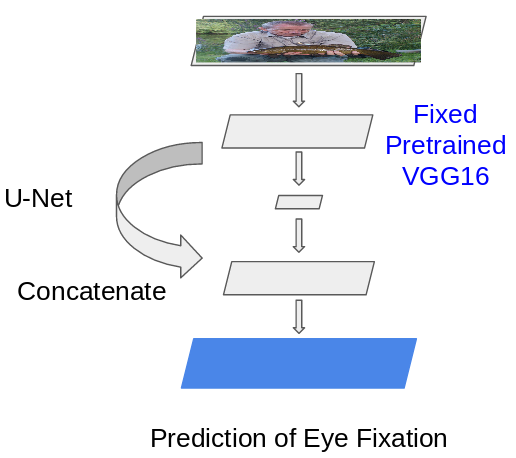
\includegraphics[width=\columnwidth]{figures/architecture_bl.png}
		
	\end{center}
	\caption{U-Net Architecture for our baseline model}
	\label{fig:short}
\end{figure*}

\subsection{Overcoming the Checkerboard Artifacts of Upsampling}
Building the upsampling using deconvolution operation introduces checkerboard artifacts, as shown in Fig. This is partly due to the overlap of the deconvolution, according to []. We overcome this by first applying a nearest-neighbor interpolation and then normal convolution operation.

\subsection{Learning Prior from the ImageNet}

 Due to the high cost of collecting eye movement data, which requires volunteers to set in front of the computer wearing an eye tracker, the number of samples in the training set is limited. We make an attempt to address this challenges by utilizing some prior knowledge of eye fixation.
 
 \begin{figure*}
 	\begin{center}
 		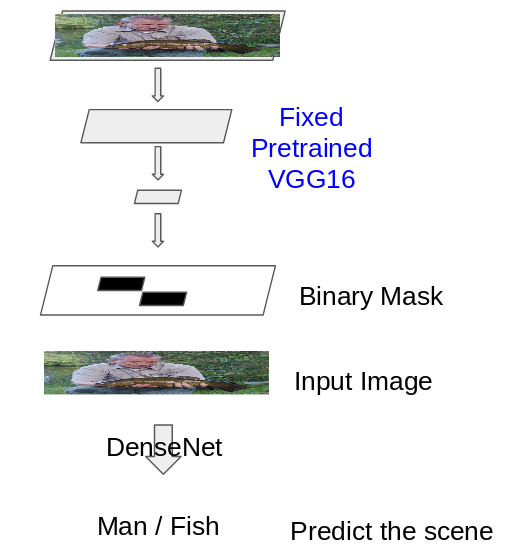
\includegraphics[width=\columnwidth]{figures/Prior.png}
 		
 	\end{center}
 	\caption{Architecture for learning the prior}
 	\label{fig:short}
 \end{figure*}
 
 We interpret eye fixation points as the places which encode the most semantic information for the image. And with this prior, we construct a model which predicts a binary mask with 0 and 1 to select the image, and then use a neural network to predict the semantic information of that after masking image. 
 
 The elements with value 1 in the predicted binary mask mimic the eye fixation point of the human, where the selection of these points should maximize the semantic information in the resulting image after training.
 
 We denote the semantic label of a given image $X$ as $y$, the predicted mask as $M$, and the loss function to minimize $L$
 $$M_i = F_1(X_i, k)$$
 $$L(X, Y) = \sum_{x_i \in X}{logP(y | F_2(M_i * x_i))}$$
 
 where * denotes element wise multiplication, $k$ denote the number of value 1 we need in the binary mask.
 
 After training The $M_i$ can be interpreted as a learned prior knowledge, which is fixed during the bayesian learning scheme.
 
 \subsection{Incorporating Prior Improves Prediction}
 
 The main contribution of our work is a bayesian inference scheme that builds upon a prior knowledge learned externally. We denote the eye fixation ground truth as $t$, 
 
 $$L = logP(M, t|x) = log(P(M|x)) + log(t|M, x)$$
 
 The prior M gives a good estimation of the eye fixation in advance, which enhance the optimization of this loss function.
 
 
 
\subsection{Training}
We train our baseline model using SGD, with learning rate of 1e-5 and weight decay of 1e-6. We train 50 epoch before we stop.

We use ImageNet data for our prior training, where the mask prediction network is based on a pretrained VGG16 network, and the network to predict semantic meaning from the masked out image is a DenseNet, which we believe have more accurate gradient information. We train this Mask prediction network using SGD with learning rate of 1e-5.


\subsection{Performance}

\begin{figure*}
\begin{center}
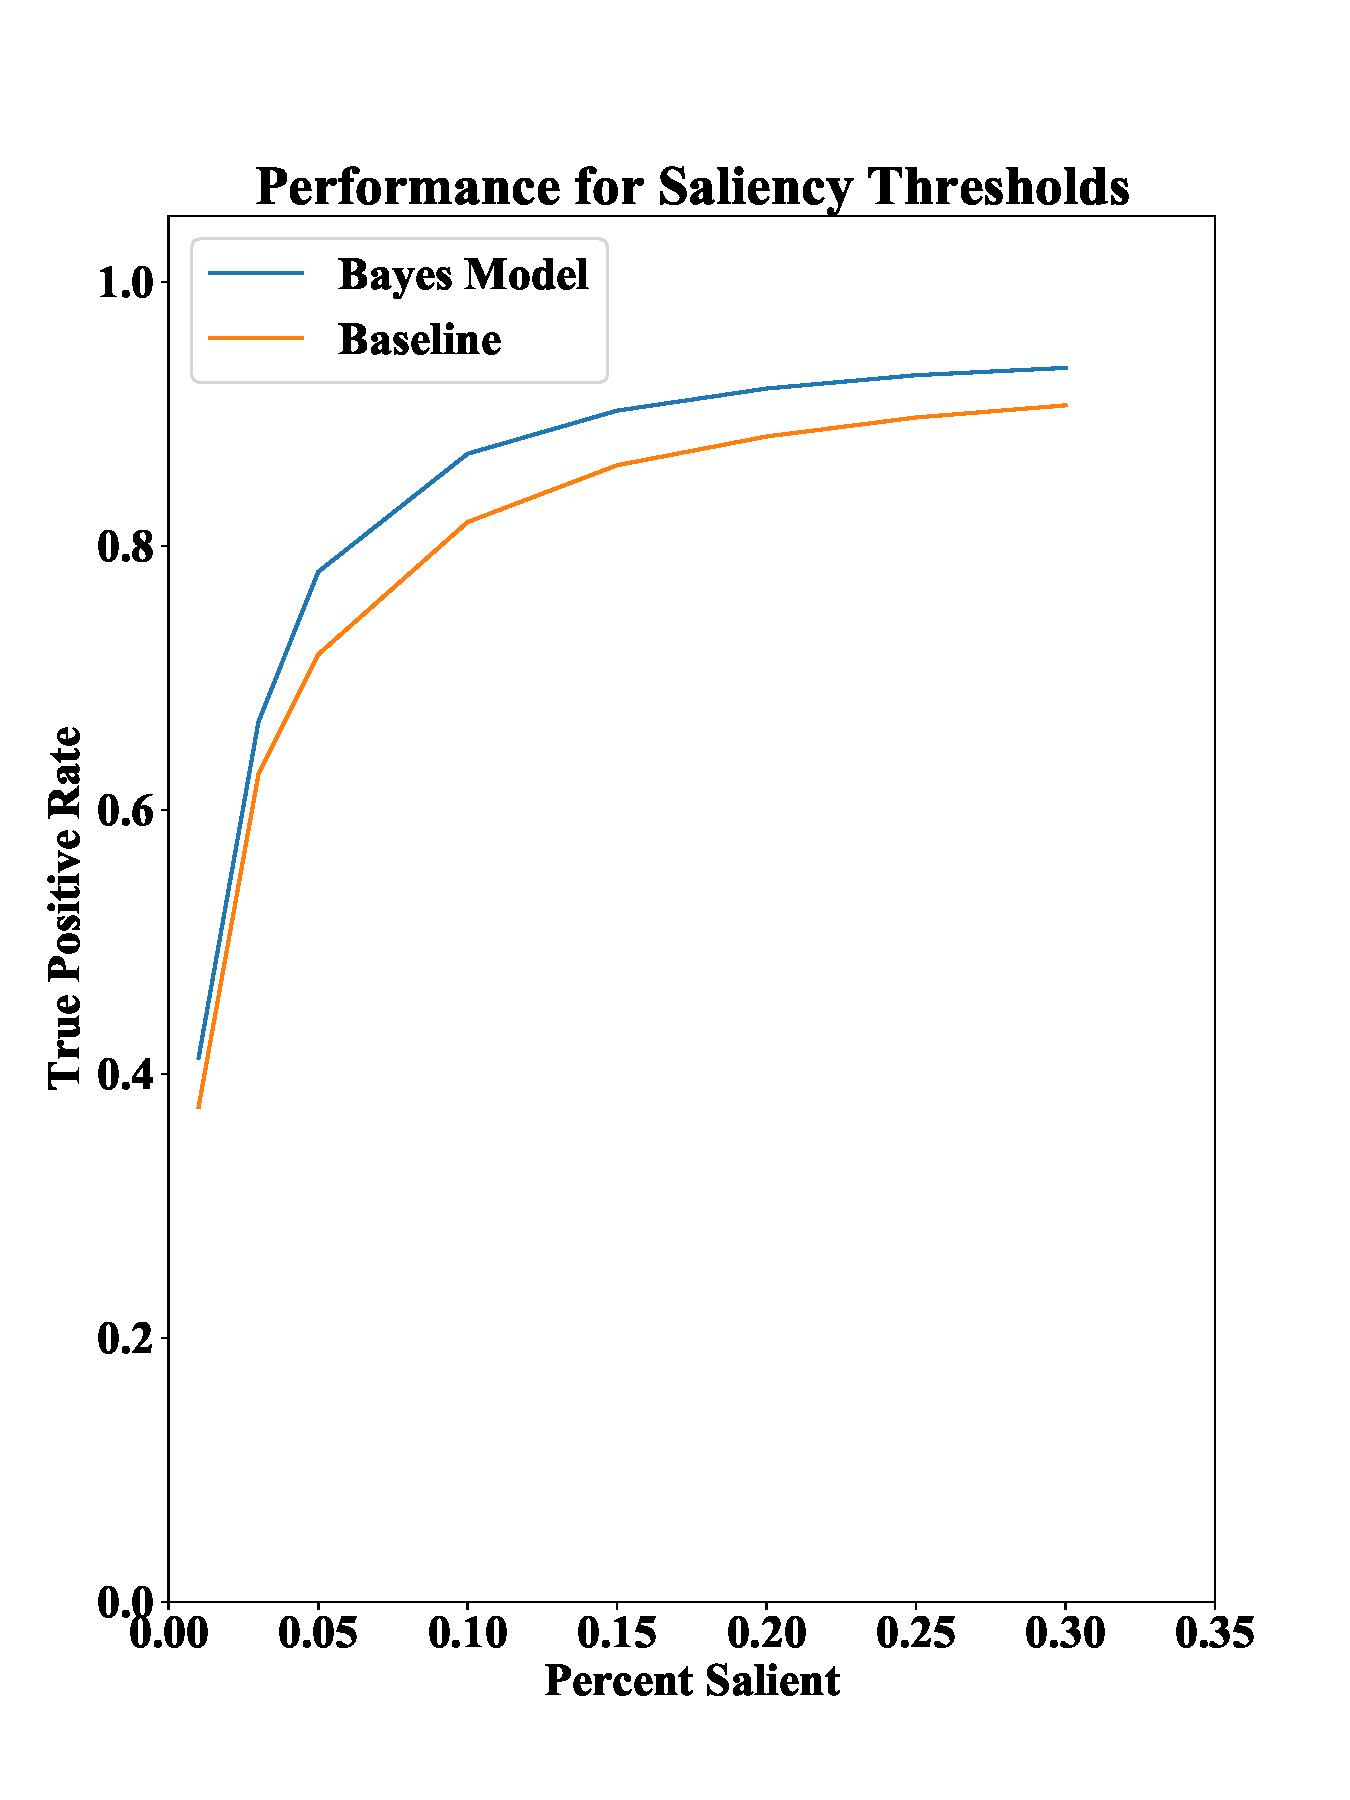
\includegraphics[width=\columnwidth]{figures/tpr.pdf}

\end{center}
   \caption{Example of a short caption, which should be centered.}
\label{fig:short}
\end{figure*}


\begin{figure*}
	\begin{center}
		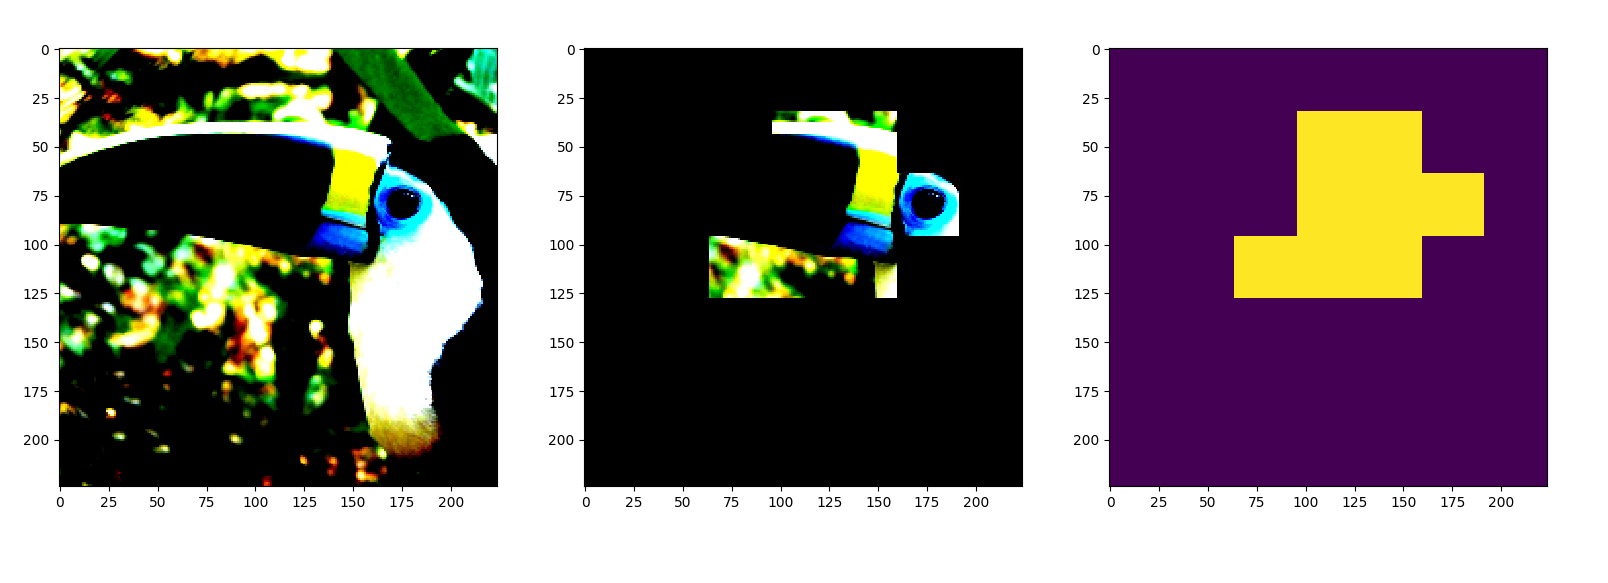
\includegraphics[width=\columnwidth]{figures/bird_mask_predict.png}
		
	\end{center}
	\caption{Example of mask learned on Imagenet}
	\label{fig:short}
\end{figure*}

\begin{figure*}
	\begin{center}
		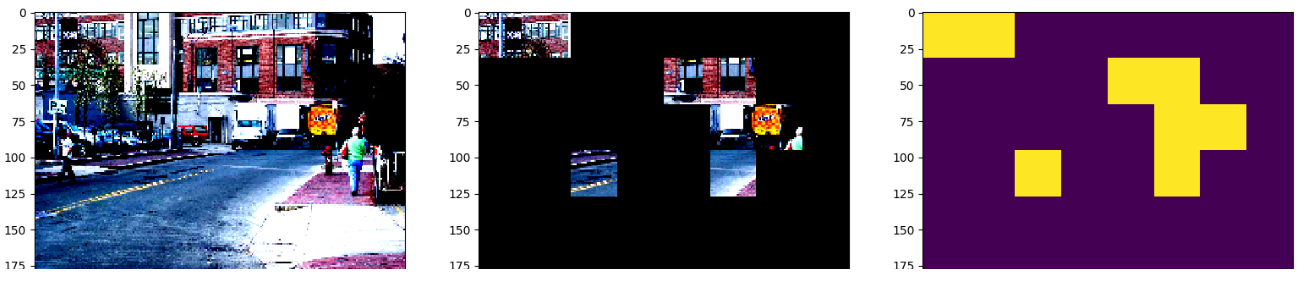
\includegraphics[width=\columnwidth]{figures/road.png}		
	\end{center}
	\caption{Example of extrapolating the prior learned on ImageNet to the eye fixation dataset}
	\label{fig:short}
\end{figure*}


\section{Conclusion}

%------------------------------------------------------------------------
{\small
\bibliographystyle{ieee}
\bibliography{egbib}
}

\end{document}
